\chapter{Revisão da Literatura}
\label{cap:02}

Este capítulo será organizado de forma a se iniciar com as formas mais primitivas e os modelos de iluminação do mais simples para o mais complexo, logo após mostrar as técnicas de sombreamento e por fim mostrar as ferramentas e trabalhos correlatos ao proposto neste

\section{Modelos de Iluminação}

Segundo \citeauthorandyear{Azevedo} o tratamento da luz é um passo essencial para visualizações realistas em ambientes tridimensionais, porém mais do que isso, os processos para chegar a tal são cada vez mais complexos conforme avançam os sistemas de hardware.

Se pensarmos em como funciona a luz no mundo real, é somente através dela que podemos enxergar qualquer coisa, pois mesmo a noite ainda recebemos a luz do sol refletida pela lua, ou seja, tudo oque vemos é somente porque os raios de luz atingem a nossa visão \cite{manssour}.

A princípio, a iluminação de forma geral necessita de uma fonte, algo que possa emitir luz, como por exemplo o sol as estrelas, uma vela ou até mesmo um fósforo. tais fontes criam uma aura ao redor que é conhecida como radiação eletromagnética, e podem emitir entre 380 a 750 nanômetros. \citeauthorandyear{Azevedo}

Porém apenas com fontes de luz a cena não se torna interessante, por isso se iniciou a iluminação de forma a ser um ponto tão longe no espaço que ilumina todos os ambientes, e para esse tipo de iluminação surgiram vários modelos.

\subsection{Reflexão Ambiente}

A luz ambiente ou reflexão ambiente é um modelo simplificado para entendermos a luz, ela utiliza padrões da realidade de forma a possibilitar a visualização de cores através da cor do objeto.

Ela "representa  um  nível  constante  de  luz  que  define  a  silhueta dos  objetos.  Esse  nível  constante  é  a  simplificação  do  modelo  de  iluminação  global proposto  por  \citeauthorandyear{Goral} que  considera  múltiplas  reflexões  da  luz  nos  diversos objetos que compõe a cena" \cite[p.~150]{Scalco2012}

De forma a esclarecer graficamente a reflexão ambiente é possível observar o modelo sendo renderizado\footnote{É o processo pelo qual se obtém imagens digitais resultantes de modelos tridimensionais} através da seguinte Figura \ref{fig:luz-ambiente}.

\begin{figure}[ht]
	\caption{Renderização usando apenas a componente ambiente.}
	\centering
	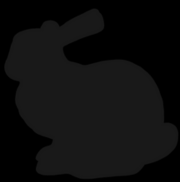
\includegraphics[scale=0.5]{imagens/09_lighting11.png}

	Fonte: \cite{Harlen_Batagelo2021}
	\label{fig:luz-ambiente}
\end{figure}


\subsection{Reflexão Difusa}

A reflexão difusa não deixa resultado sombras no ambiente, isso acontece porque a luz difusa provém de diferentes posições criando um volume no objeto sem sombras a sua volta, essa ideia foi feita a partir do \citeauthorandyear{alcalde2012interaccion} e um estudo de luzes em superfícies rugosas.

Matematicamente, falando podemos utilizar dos estudos de \cite{SteveMarschner584} Quando uma superfície lambertiana\footnote{De forma controlada e uniforme, a superfície lambertiana reflete uniformemente a luz, independentemente da direção em que a luz é refletida. } é iluminada, a luz que incide sobre o ponto P é refletida uniformemente em todas as direções.  Isso é ilustrado na figura \ref{fig:reflexão difusa} a seguir.

\begin{figure}[ht]
	\caption{Reflexão difusa ideal.}
	\centering
	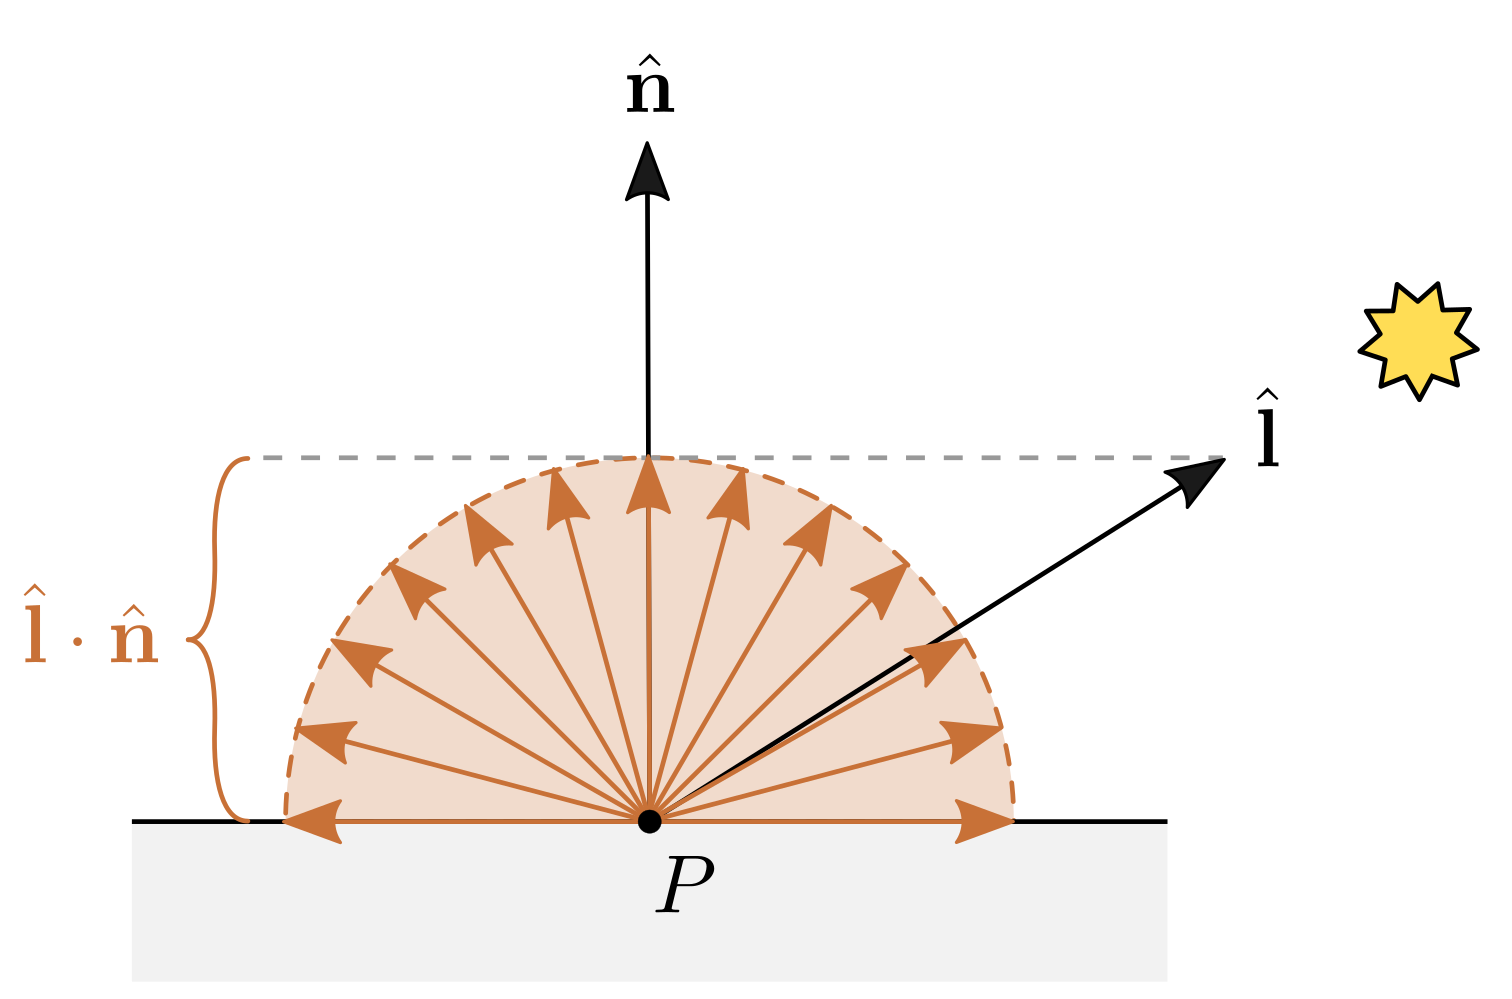
\includegraphics[scale=0.8]{imagens/09_lighting9.png}

	Fonte: \cite{Harlen_Batagelo2021}
	\label{fig:reflexão difusa}
\end{figure}

\subsection{Reflexão Especular}

"a iluminação especular identifica os realces especulares brilhantes que ocorrem quando a luz atinge uma superfície de objeto e reflete de volta em direção à câmera. A iluminação especular é mais intensa do que a luz difusa e incide mais rapidamente na superfície do objeto." dito por \cite{Steven2022}

É possível dizer que a partir de  uma superfície perfeitamente especular é semelhante a um espelho ideal.  Se a luz atinge o ponto P, ela é refletida apenas na direção reflexa \begin{math}\hat{r}\end{math} do vetor \begin{math}\hat{l}\end{math}  em torno de \begin{math}\hat{n}\end{math} .  Isso é ilustrado na Figura \ref{fig:reflexão especular}.

\begin{figure}[ht]
	\caption{Reflexão especular ideal.}
	\centering
	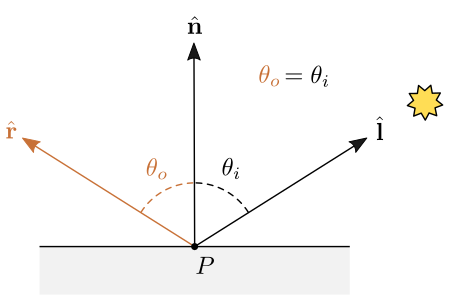
\includegraphics[scale=0.7]{imagens/09_lighting14.png}

	Fonte: \cite{Harlen_Batagelo2021}
	\label{fig:reflexão especular}
\end{figure}

\section{Sombreamento}

De acordo com \citeauthorandyear{Harlen_Batagelo2021} "Sombreamento ou tonalização (do inglês \textit{shading}) é o processo de modificar a intensidade das cores de uma imagem através de tons claros e escuros, de modo a produzir a percepção de volume e profundidade de um objeto tridimensional."

\subsection{Flat Shading}

O sombreamento plano está em sua eficiência. A frequência de cálculo do modelo de iluminação é diretamente proporcional ao número de faces, que geralmente é menor que o número de \textit{pixels}, resultando em menos avaliações.

Segundo o \citeauthorandyear{SteveMarschner584} O sombreamento plano geralmente expõe as arestas irregulares de uma malha poligonal, resultando em uma aparência fragmentada. Isso pode ser um efeito atraente se o objeto em questão for um poliedro. No entanto, se a malha pretende aproximar uma superfície lisa, o resultado desejado só pode ser alcançado dividindo a malha em faces menores. Neste exemplo, uma malha triangular atua como uma imitação de uma esfera. Ao aumentar o número de subdivisões, é fácil ver que os intervalos de luz entre as faces são equilibrados suavemente.

Atualmente, o uso de sombreamento plano na GPU\footnote{\textit{Graphics Processing Unit}, ou unidade de processamento de gráficos} não melhora a eficiência da renderização. Isso ocorre porque o pipeline gráfico atual é otimizado para lidar com atributos de vértice em vez de atributos de triângulo.

\subsection{Sombreamento de Gourand}

A suavização das transições de luz entre as faces dá ao sombreamento Gouraud uma vantagem sobre a técnica de sombreamento plano, pois melhora significativamente o aspecto visual de um objeto, superando visualmente sua contraparte com igual número de faces.  Embora digno de nota, o efeito visual apelidado de bandas de Mach\footnote{O físico Ernst Mach se deparou com esse fenômeno na década de 1860, que pode ser atribuído a um contraste elevado das bordas em tons de cinza.} geralmente faz com que as bordas dos rostos pareçam mais pronunciadas do que a área interna. Isso é importante para que as imagens possam ser retratadas como objetos realistas em desenhos, esse efeito resulta do contraste exagerado criado nas bordas, que o sistema visual humano detecta facilmente com base na obra de \citeauthorandyear{Gourand1971-gs}

Onde faltam vértices de malha, pode haver um efeito de brilho cintilante, causado pela perda de brilho especular.  Outro problema que pode ser enfrentado com o sombreamento Gouraud é essa ocorrência.  Para aliviar isso, pode-se aumentar o número de refinamentos de malha, embora isso possa aumentar o tempo de processamento.  Se as subdivisões forem baixas, há uma chance de encontrar esse problema como mostrado por \citeauthorandyear{Harlen_Batagelo2021}

Calcular o vetor normal do vértice é uma etapa crucial na utilização do sombreamento de Gouraud, pois ele pode ser obtido tomando-se a média dos vetores normais da face próxima.

\subsection{Sombreamento de Phong}

Segundo \cite{Gomes_undated-tr} No método de sombreamento de Phong, a partir das normais aos vértices, realizada do mesmo modo que o sombreamento de Gourand retratado abaixo, é calculada a normal a cada quadrícula através da interpolação das normais.isto é então usada no modelo de iluminação de Phong para calcular a intensidade da energia luminosa reflectida.
\citeauthorandyear{Harlen_Batagelo2021} Explica que o sombreamento de Phong é que exige mais dos sombreamentos, e consiste em avaliar a equação do modelo de iluminação para cada fragmento. O resultado é muito superior ao sombreamento de Gouraud para um mesmo número de faces. \citeauthorandyear{SteveMarschner584} retrata que para o modelo de Phong precisamos calcular um vetor \begin{math}\hat{n}\end{math} para cada fragmento. Isso geralmente ocorre da interpolação linear das coordenadas (x,y,z) dos vetores normais de vértice, igual aos componentes RGB das cores dos vértices são interpoladas para criar um degradê de cores. Porem, neste caso, o vetor de coordenadas interpoladas é normalizado novamente no \textit{fragment shader}\footnote{através da openGL} para ser utilizado como vetor \begin{math}\hat{n}\end{math} da equação.

No sombreamento de Phong, as bandas de Mach são praticamente imperceptíveis. Além disso, o brilho especular é mantido independentemente do refinamento da malha.


\section{Segment Anything em Visão Computacional}

O modelo Segment Anything (SA) é um avanço crucial na segmentação de imagens, capaz de produzir mais de um bilhão de máscaras em 11 milhões de imagens. Sua flexibilidade permite sua aplicação em diversas áreas, como a imagem médica e a glaciologia, devido à sua capacidade de executar tarefas zero-shot, muitas vezes superando métodos supervisionados. O SA utiliza redes neurais convolucionais (CNNs), uma arquitetura codificadora-decodificadora e mecanismos de atenção espacial para alcançar alta eficiência. No entanto, sua complexidade representa um desafio para implementação em tempo real e em ambientes com recursos limitados \cite{kirillov2023segany}.
Em campos específicos, como microscopia e glaciologia, o SA foi adaptado para melhorar a qualidade da segmentação em diversas condições de imagem, evidenciando sua robustez e versatilidade \cite{zhongkai_yuan_2024}. 
Por exemplo, sua adaptação para dados de microscopia levou a melhorias significativas na segmentação e rastreamento de objetos em múltiplas dimensões, destacando o potencial do modelo para resolver problemas complexos em análise de imagens \cite{anwai_archit__2023}.

\subsection{Codificador de Imagens (Image Encoder)}

O codificador de imagens utilizado pode ser qualquer rede que produza uma incorporação (embedding) da imagem com dimensões \(C \times H \times W\). Para garantir escalabilidade e acesso a um pré-treinamento robusto, é empregado um Vision Transformer (ViT) pré-treinado com MAE, especificamente um ViT-H/16. Este ViT-H/16 possui atenção em janelas de \(14 \times 14\) e quatro blocos de atenção global igualmente espaçados. A saída do codificador é uma incorporação reduzida em \(16\times\) da imagem de entrada, a qual possui uma resolução de entrada de \(1024 \times 1024\), resultando em uma incorporação final de \(64 \times 64\).

Para reduzir a dimensão dos canais, é aplicada uma convolução \(1 \times 1\) para alcançar 256 canais, seguida de uma convolução \(3 \times 3\) também com 256 canais. Ambas as convoluções são seguidas por uma normalização em camadas (\textit{Layer Normalization}).

\subsection{Codificador de Prompts (Prompt Encoder)}

Prompts esparsos são mapeados para incorporações vetoriais de 256 dimensões. Pontos são representados como a soma de uma codificação posicional da localização do ponto e de uma incorporação aprendida que indica se o ponto está no primeiro plano ou no fundo. Caixas são representadas por um par de incorporações: uma para o canto superior esquerdo e outra para o canto inferior direito, utilizando codificações posicionais e incorporações aprendidas.

Para representar texto livre, é utilizado o codificador de texto do CLIP, com a possibilidade de utilizar qualquer codificador de texto. Prompts densos, como máscaras, possuem correspondência espacial com a imagem e são inseridos em uma resolução \(4\times\) menor do que a imagem de entrada. Estas máscaras são então reduzidas adicionalmente \(4\times\) usando convoluções \(2 \times 2\), resultando em uma dimensão de canal final de 256, com ativações GELU e normalização em camadas entre as etapas.

\subsection{Decodificador de Máscaras (Lightweight Mask Decoder)}

O decodificador de máscaras é um módulo eficiente que mapeia a incorporação da imagem e um conjunto de incorporações de prompt para uma máscara de saída. Para combinar essas entradas, nos inspiramos em modelos de segmentação baseados em Transformer \cite{DBLP:journals/corr/abs-2005-12872}\cite{NEURIPS2021_950a4152} e modificamos um decodificador Transformer padrão \cite{DBLP:journals/corr/VaswaniSPUJGKP17}. Antes de aplicar nosso decodificador, inserimos no conjunto de incorporações de prompt um token de saída aprendido, que será utilizado na saída do decodificador, de forma análoga ao token [class] descrito em \cite{DBLP:journals/corr/VaswaniSPUJGKP17}. Para simplificar, referimos a essas incorporações (excluindo a incorporação da imagem) coletivamente como “tokens”.

Para garantir que o decodificador tenha acesso a informações geométricas críticas, as codificações posicionais são adicionadas à incorporação da imagem sempre que participam de uma camada de atenção. Além disso, os tokens de prompt originais completos (incluindo suas codificações posicionais) são re-adicionados aos tokens atualizados sempre que participam de uma camada de atenção. Isso permite uma forte dependência tanto da localização geométrica quanto do tipo do token de prompt.

Após a execução do decodificador, ampliamos a incorporação da imagem atualizada em \(4\times\) usando duas camadas convolucionais transpostas (resultando em uma escala \(4\times\) menor em relação à imagem de entrada). Em seguida, os tokens realizam uma última atenção para a incorporação da imagem, e passamos a incorporação do token de saída atualizada para uma pequena MLP de três camadas que gera um vetor correspondente à dimensão de canal da incorporação da imagem ampliada. Finalmente, prevemos uma máscara através de um produto ponto a ponto espacial entre a incorporação da imagem ampliada e a saída da MLP.

O Transformer utiliza uma dimensão de incorporação de 256. Os blocos MLP do Transformer têm uma grande dimensão interna de 2048, mas a MLP é aplicada apenas aos tokens de prompt, que são relativamente poucos (raramente ultrapassando 20). No entanto, em camadas de cross-atenção, onde temos uma incorporação de imagem de \(64 \times 64\), reduzimos a dimensão do canal das queries, keys, e values em \(2\times\) para 128, visando eficiência computacional. Todas as camadas de atenção utilizam 8 cabeças.

As convoluções transpostas usadas para ampliar a incorporação da imagem de saída são \(2 \times 2\), com stride 2 e dimensões de canal de saída de 64 e 32, e utilizam ativações GELU. Elas são separadas por normalização em camadas.


\section{Geração de Mapas de Normais}

Os mapas de normais são essenciais para definir como a luz interage com as superfícies, criando efeitos de iluminação dinâmica em gráficos 3D, pixel art e renderização de fluidos. A geração de mapas de normais, especialmente para pixel art, é desafiadora devido à sua estética única. Métodos como amostragem geométrica e modelos generativos profundos, como Redes Adversárias Generativas Condicionais (CGANs), foram desenvolvidos para gerar mapas de normais precisos. Um estudo compilou diferentes técnicas de geração de mapas de normais e analisou sua aplicabilidade ao pixel art, contribuindo para uma análise qualitativa do comportamento dessas técnicas em diferentes cenários \cite{Moreira}.
No contexto de renderização de fluidos, a refinada representação dos mapas de normais por meio de redes neurais aprimora a qualidade da renderização, mantendo detalhes e suavidade. 
O uso de CGANs tem demonstrado eficácia em melhorar a precisão dos mapas de normais, capturando detalhes intricados e aprimorando a iluminação realista em renderizações \cite{myungjin_choi__2021}. 
A integração dessas técnicas na ferramenta proposta no seu TCC pode aprimorar a percepção de profundidade e a iluminação realista em aplicações de imagens.

\subsection{Métodos Tradicionais}

Os mapas de normais são amplamente utilizados para simular detalhes de superfícies sem a necessidade de adicionar geometria adicional a um modelo 3D.
Um método tradicional de gerar mapas de normais é a partir de malhas 3D de alta resolução. 
Nesta abordagem, um modelo detalhado é projetado em uma malha de menor resolução, e a diferença nas inclinações das superfícies é codificada em um mapa de normais.
Outro método convencional é o bump mapping, que utiliza mapas de normais para simular rugosidades e imperfeições na superfície de um objeto 3D, proporcionando a ilusão de detalhes sem alterar a malha subjacente. 
Embora essas técnicas sejam eficazes, elas possuem limitações, especialmente quando aplicadas a estilos gráficos mais estilizados, como o pixel art, ou quando a resolução das imagens é baixa. 
Em tais casos, os métodos tradicionais podem não capturar corretamente as nuances da superfície ou podem introduzir artefatos visuais, resultando em uma renderização menos realista. 
Por exemplo, a análise de \cite{Moreira} destaca que a aplicação desses métodos em pixel art pode não produzir resultados precisos devido às especificidades do estilo.
Essas desvantagens motivaram o desenvolvimento de técnicas mais avançadas, que buscam superar os limites das abordagens tradicionais e oferecer soluções mais adaptáveis a diferentes estilos e cenários.

\section{Técnicas avançadas de pixel arte}

A geração de mapas de normais para pixel art apresenta desafios únicos devido à natureza estilizada e à baixa resolução desse tipo de arte.
Métodos tradicionais muitas vezes falham em capturar os detalhes necessários para representar corretamente a interação da luz com a superfície pixelada.
Uma técnica avançada para abordar esse problema é a amostragem geométrica, que se concentra na análise da forma geométrica dos pixels para criar mapas de normais mais precisos \citeyear{yi_he__2021}. 
Além disso, o uso de Redes Adversárias Generativas Condicionais (CGANs) oferece uma abordagem inovadora para a geração de mapas de normais em pixel arte, permitindo a produção de resultados mais refinados e detalhados. 
Por exemplo, \citeyear{Su2018} desenvolveram um sistema interativo que utiliza técnicas de deep learning para gerar mapas de normais de alta qualidade a partir de esboços, melhorando a precisão e a interatividade do processo. 
Essas redes utilizam amostras geométricas para treinar modelos capazes de gerar mapas de normais que respeitam as características visuais do pixel arte, como bordas nítidas e transições suaves de luz. No contexto de renderização de fluidos, abordagens baseadas em aprendizado profundo, como a proposta por \citeyear{myungjin_choi__2021}, refinam os mapas de normais para aprimorar a qualidade da renderização, preservando detalhes e suavidade. 
Essas técnicas avançadas são essenciais para garantir que a iluminação e a profundidade sejam representadas de forma precisa, resultando em uma renderização mais realista e visualmente atraente.

\section{Ferramentas para iluminação de cenários}

Para a iluminação ser feita em ambiente gráfico foram criadas diversas ferramentas, dentre elas Vulkan e OpenGL, que trabalham em cima de toda a forma como a luz e os materiais funcionam no ambiente, proporcionando configurações avançadas de baixo nível para que exista controle total do ambiente sendo desenvolvido.

\subsection{Vulkan}

Segundo o \cite{Khronos_Group2016-ir}, a Vulkan\footnote{disponível: https://www.vulkan.org/} é uma API \footnote{ Application Programming Interface } de gráficos de baixo nível, criada pela Khronos Group, com o objetivo de fornecer aos desenvolvedores um acesso mais direto ao hardware do computador para criar aplicativos gráficos de alto desempenho em várias plataformas e dispositivos. Ela pode ser usada para desenvolver aplicativos para diversos casos de uso. Embora as aplicações em Vulkan possam escolher usar um subconjunto das funcionalidades descritas abaixo, a API foi projetada para que um desenvolvedor possa usar todas elas em uma única API.multiplataforma.

\subsection{OpenGL}
OpenGL\footnote{disponível: https://www.opengl.org/} é uma biblioteca de renderização. No entanto, o que o OpenGL não faz é reter informações sobre um "objeto". Tudo o que o OpenGL vê é uma esfera de polígonos e um conjunto de estados com os quais renderizá-los. não se lembra que foi desenhado uma linha em um local determinado e uma esfera em outro.

Por causa disso, a maneira geral de usar o OpenGL é desenhar tudo o que você precisa desenhar e, em seguida, mostrar essa imagem com um comando de troca de \textit{buffer} dependente da plataforma. Se você precisar atualizar a imagem, desenhe tudo novamente, mesmo que precise atualizar apenas parte dela. Se você quiser animar objetos se movendo na tela, precisa de um \textit{loop} que constantemente limpe e redesenhe a tela.

\subsection{Engines}

Está sessão tem o intuito de apresentar as \textit{engines} do mercado atual, afinal elas tem sua própria forma de criar iluminação e alterar de diversas maneiras para atender a um estilo visual único com \textit{shaders} ou outros efeitos.

De acordo com \cite{Felipe2017-av} Em sua essência, a \textit{engine} é um \textit{software}  vital que compila todos os arquivos e bibliotecas essenciais dos quais um jogo depende. Essa ferramenta serve como base para o desenvolvimento de jogos, permitindo que os desenvolvedores criem habilmente sua visão.  No entanto, a criação de jogos requer muito mais do que apenas um mecanismo.  Os desenvolvedores também devem fazer uso de editores de imagem, software de áudio e vídeo, modeladores 3D e software vetorial, dependendo da situação.  Uma vez criados, esses elementos ganham vida dentro do motor, onde recebem animação, física, efeitos sonoros e outros recursos cruciais.

\subsubsection{Unity}
A marca registrada do \href{https://unity.com/pt}{\textit{Unity}} reside em seu estilo de programação, utilizando de vários objetos conectando vários pontos em um mesmo código. Distinto e estrutura de projeto que possui uma simplicidade inigualável.  O \textit{Unity} permite que os desenvolvedores utilizem as alternativas disponíveis e abre vários caminhos para os criadores se concentrarem em seus conhecimentos, principalmente na conduta dos personagens, de ambas as classes segundo \cite{Henrique2014-ka}

Embora o \textit{Unity} tenha um objetivo de desenvolvimento bem definido, seus recursos se estendem além disso para diversos tipos de projeto.  Gráficos altamente realistas são a combinação perfeita para jogos de aventura como RPGs \footnote{Role Playing Game ou Jogo de interpretação de personagem}, TPSs \footnote{Third Person Shooter ou Tiro em terceira pessoa} e FPSs \footnote{First Person Shooter ou Tiro em primeira pessoa} ao usar o \textit{Unity}.  A capacidade de incorporar elementos feitos por outros desenvolvedores de jogos aos nossos é um dos maiores pontos fortes do \textit{Unity}.  Essa funcionalidade é tremendamente vantajosa para indivíduos sem habilidades gráficas extensas, como modelagem 3D ou ilustração.

\subsubsection{Godot}

De acordo com \citeonline{Juan_Linietsky},na \href{https://unity.com/pt}{Godot} você tem liberdade criativa para personalizar o código-fonte do mecanismo de jogo, totalmente adaptado às suas necessidades.  O software é flexível no sentido de que pode facilmente gerar jogos 2D e 3D, com uma abundância de recursos como gráficos, som, física e animação.  Além disso, sua compatibilidade entre plataformas se estende a \textit{Windows}, macOS, Linux, Android, iOS e \textit{web}.

Comparado a outros mecanismos de jogos de código aberto, o Godot se destaca por sua interface amigável e processo de aprendizado simples.  Com documentação abrangente, os aspirantes a criadores de jogos podem mergulhar direto no processo de criação do jogo.  Os jogadores também podem fazer sua programação em várias linguagens diferentes, incluindo CSharp e GDScript.  Esse recurso torna mais fácil para os desenvolvedores selecionarem o idioma de sua preferência.

\section{Trabalhos Correlatos}

Nesta seção são apresentados os trabalhos correlatos ao proposto neste trabalho

\subsection{Geração De Mapas De Iluminação Baseado Em Topologia Estimada Para Iluminação De Sprites}

Este trabalho de autoria \citeauthorandyear{abraao2017} trata-se de uma pesquisa prática em torno do mapeamento de uma imagem, e criação de uma topologia, no âmbito das pixel artes atualmente esse processo de iluminação é realizada de duas formas, com modelos em 3D ou de forma manual, mas o que realmente é tratado desse trabalho é de como esse tipo de tecnologia pode facilitar a vida do profissional.

Em seu desenvolvimento é retratado métodos já criados para tentar resolver o problema, um deles é o \textit{Cross Shade} proposto por \cite{Shao2012} que cria em um desenho uma especie de cruz para que em cada plano do desenho possa ser identificado a sua normal de forma como a cruz está, pegando sua curvatura para identificar um objeto em três dimensões

Dentre os métodos é utilizado para os resultados uma criação de mapa topológico a partir da ferramenta \textit{sprite illuminator} e algumas customizações por cima do que foi gerado para que fosse possível uma bom resultado em pixel artes bem pequenas.

\subsection{Analysis and Compilation of Normal Map Generation Techniques for Pixel Art}

Esse trabalho do autor \citeonline{Moreira} tem como influencia a luz que interage com cada pixel do material. Existem vários métodos para gerar mapas normais em jogos 3D, mas aplicá-los na arte pixel pode não produzir resultados precisos por causa das particularidades do estilo. Este trabalho reúne diferentes métodos de geração de mapas normais e estuda sua aplicação na arte pixel, contribuindo para uma análise qualitativa do comportamento desses métodos em diferentes estudos de caso e diminuindo a escassez de material existente sobre essas técnicas.

\subsection{CrossSketch: freeform surface modeling with details}

Este artigo do autor \citeonline{Alexis} apresenta uma nova técnica para modelar uma superfície tridimensional livre, incluindo sua forma global e pequenos detalhes, usando uma interface de desenho a partir de um único ponto de vista. Em sistemas de modelagem anteriores que utilizavam esboços como entrada, a forma era reconstruída a partir da silhueta e o usuário tinha pouco controle sobre as partes internas do resultado. É gerado uma grade de linhas co-planas a partir de um pequeno número de traços desenhados pelo usuário,foi estimado o vetor normal onde ele é restrito e formamos a superfície propagando essa informação para toda a grade. Como resultado, traços menores atuam localmente para adicionar detalhes, enquanto traços maiores modificam toda a superfície. Esse trabalho oferece uma nova abordagem para o problema de modelagem a partir de esboços e tem a intenção de ser parte de um sistema de modelagem mais complexo.